\section{Problem 1}

\subsection{Question 1}

Suppose we have a $v$ distributed in domain, 
we have:
\begin{equation}
    \label{initial equation}
    \int_\Omega (-\Delta u - f)(u-v)\mathrm{d}\Omega = 0
\end{equation}
considering an arbitrary $w$, we use integrate by part:
\begin{equation}
    \label{integrate by part}
    \int_\Omega w\Delta u \mathrm{d}\Omega = 
    \int_{\partial \Omega} w\frac{\partial u}{\partial n} \mathrm{d}\Gamma -
    \int_\Omega \nabla w \cdot \nabla u \mathrm{d}\Omega
\end{equation}
and by Cauchy-Schwarz inequality:
\begin{equation}
    \label{Cauchy-Schwarz inequality}
    \int_\Omega \nabla w \cdot \nabla u \mathrm{d}\Omega \leq
    \frac{1}{2}
    \left(\int_\Omega \nabla w \cdot \nabla w \mathrm{d}\Omega +
    \int_\Omega \nabla u \cdot \nabla u \mathrm{d}\Omega\right)
\end{equation}
apply (\ref{integrate by part}) to (\ref{initial equation}), we have:
\begin{equation}
    \begin{aligned}
        -\int_\Omega u \nabla^2 u \mathrm{d}\Omega + 
        \int_\Omega v \nabla^2 u \mathrm{d}\Omega -
        \int_\Omega f u \mathrm{d}\Omega +
        \int_\Omega f v \mathrm{d}\Omega &=0\\
        \int_\Omega \nabla u \cdot \nabla u \mathrm{d}\Omega -
        \int_{\partial \Omega} u\frac{\partial u}{\partial n} \mathrm{d}\Gamma -
        \int_\Omega f u \mathrm{d}\Omega &=\\
        \int_\Omega \nabla v \cdot \nabla u \mathrm{d}\Omega-
        \int_{\partial \Omega} v\frac{\partial u}{\partial n} \mathrm{d}\Gamma &-
        \int_\Omega f v \mathrm{d}\Omega\\
        \int_\Omega \nabla u \cdot \nabla u \mathrm{d}\Omega -
        \int_{\partial \Omega} u\bar{t} \mathrm{d}\Gamma -
        \int_\Omega f u \mathrm{d}\Omega &=\\
        \int_\Omega \nabla v \cdot \nabla u \mathrm{d}\Omega-
        \int_{\partial \Omega} v\bar{t} \mathrm{d}\Gamma &-
        \int_\Omega f v \mathrm{d}\Omega\\
    \end{aligned}
\end{equation}
apply (\ref{Cauchy-Schwarz inequality}) above,
we will have:
\begin{equation}
    \begin{aligned}
        \int_\Omega \nabla u \cdot \nabla u \mathrm{d}\Omega -
        \int_{\partial \Omega} u\bar{t} \mathrm{d}\Gamma -
        \int_\Omega f u \mathrm{d}\Omega &\leq\\
        \frac{1}{2}\int_\Omega (\nabla u\cdot \nabla u + \nabla v\cdot \nabla v) \Omega-
        \int_{\partial \Omega} v\bar{t} \mathrm{d}\Gamma &-
        \int_\Omega f v \mathrm{d}\Omega\\
    \end{aligned}
\end{equation}
denote $U[w]$ as below:
\begin{equation}
    U[w]=
    \int_\Omega \frac{1}{2}\nabla w\cdot \nabla w \mathrm{d}\Omega-
    \int_{\partial \Omega} w\bar{t} \mathrm{d}\Gamma -
    \int_\Omega f w \mathrm{d}\Omega
\end{equation}
we will have:
\begin{equation}
    U[u] \leq U[v]
\end{equation}
finally we reduce the Poisson equation to a minimization problem,
and the solution of the Poisson equation is the minimizer of $U[u]$.

\subsection{Question 2}

From integral by part(\ref{integrate by part}), we have:
\begin{equation}
    \begin{aligned}
        \int_\Omega \nabla w\cdot \nabla\tilde{u}\mathrm{d}\Omega&=
    \int_{\partial \Omega} w\frac{\partial \tilde{u}}{\partial n}\mathrm{d}\Gamma-
    \int_\Omega w\Delta \tilde{u}\mathrm{d}\Omega\\
    \end{aligned}
\end{equation}
thus we have:
\begin{equation}
    \int_\Omega w(-\Delta \tilde{u}-f)\mathrm{d}\Omega+
    \int_{\partial \Omega} w\left(
        \frac{\partial \tilde{u}}{\partial n}-\bar{t}
    \right)\mathrm{d}\Gamma=0
\end{equation}
when $w=0$ at $\partial \Omega$, we have:
\begin{equation}
    \int_\Omega w(-\Delta \tilde{u}-f)\mathrm{d}\Omega=0
\end{equation}
for the arbitrary $w$, we have:
\begin{equation}
    -\Delta \tilde{u}-f=0
\end{equation}

Consider $\psi=\tilde{u}-u$, which satisfies:
\begin{equation}
    \nabla^2 \psi=0 \quad \text{in} \quad \Omega, \quad\psi=0 \quad \text{on} \quad \partial \Omega
\end{equation}
thus:
\begin{equation}
    0=\int_\Omega \psi\nabla^2 \psi \mathrm{d}\Omega=
    \int_{\partial \Omega} \psi\frac{\partial \psi}{\partial n}\mathrm{d}\Gamma-
    \int_\Omega \nabla \psi\cdot \nabla \psi \mathrm{d}\Omega
\end{equation}
we will have:
\begin{equation}
    \nabla\psi=\vec{0} \quad \text{in} \quad \Omega
\end{equation}
for $\psi=0$ at $\partial \Omega$, we have:
\begin{equation}
    \psi=0 \quad \text{in} \quad \Omega
\end{equation}
which indicates that $\tilde{u}=u$.

\subsection{Question 3}

\begin{figure}[H]
    \centering
    \begin{tikzpicture}
        \draw (0, 0)--(4, 0)--(0, 4)--(0, 0);
        \node at (-1.2, 2) {$\vec{n}\cdot \nabla u=1$};
        \node at (2, -0.5) {$u=0$};
        \node at (3.2, 2) {$\vec{n}\cdot \nabla u=0$};

        \draw[dashed] (0,0)--(0,-1);
        \draw[dashed] (4,0)--(4,-1);
        \draw[<->] (0,-0.8)--(4,-0.8);
        \node at (2, -1.5) {$2$};

        \draw[dashed] (0,4)--(5,4);
        \draw[dashed] (0,0)--(5,0);
        \draw[<->] (4.8,0)--(4.8,4);
        \node at (5, 2) {$2$};
    \end{tikzpicture}
    \caption{fig: Problem Setting}
\end{figure}

Considering a shape function $\phi_i$ in single triangular element,
we have:
\begin{equation}
    \sum_j a_j \int_{\Omega_e} \nabla \phi_i \cdot \nabla \phi_j \mathrm{d}\Omega=
    \int_{\partial \Omega_e} \phi_i \frac{\partial u}{\partial n} \mathrm{d}\Gamma
\end{equation}

Let's consider an element as below:
\begin{figure}[H]
    \centering
    \begin{tikzpicture}
        \draw (0, 0)--(2, 1)--(0, 3)--(0, 0);
        % bold
        \draw[red, thick] (0, 0)--(0, 3);
        \node at (-0.5, 0) {$1, \phi_1$};
        \node at (2.5, 1) {$2, \phi_2$};
        \node at (-0.5, 3) {$3, \phi_3$};

        \node at (-2, 1.5) {$\vec{n}\cdot \nabla u=t$};
    \end{tikzpicture}
    \caption{fig: Single Element with Neumann Boundary Condition}
\end{figure}

we will have the integral as below:
\begin{equation}
    \begin{aligned}
        \int_3^1 \phi_2 t dl &= 0\\
        \int_3^1 \phi_1 t dl &= \frac{t}{2}l_{13}\\
        \int_3^1 \phi_3 t dl &= \frac{t}{2}l_{13}\\
    \end{aligned}
\end{equation}
this integral seems to devide part $tl_{13}$ into two parts,
which are added separately to node 1 and node 3.

\textbf{You may read the report last year in folder 'FEM/Autumn2022' for more details 
of the derivation of the integral.
Another option is to watch video bilibili:
https://www.bilibili.com/video/BV1qD4y1J7ZU/?spm
\_id\_from=333.999.0.0,
a video by me on last year's homework.}

Generally, we have:
\begin{equation}
    \left[\sum_e \int_{\Omega_e} \nabla \phi_i^e \cdot \nabla \phi_j^e \mathrm{d}\Omega\right]
    (\tilde{u}+u_\Gamma)=
    \left[
        \sum_e \int_{\partial \Omega_e} \phi_i^e \frac{\partial u}{\partial n} \mathrm{d}\Gamma
    \right]
\end{equation}

\subsubsection{MMA Solution}

To verify the solution by hand-writing code, 
we use Mathematica to solve the problem first.
The notebook is printed as below:

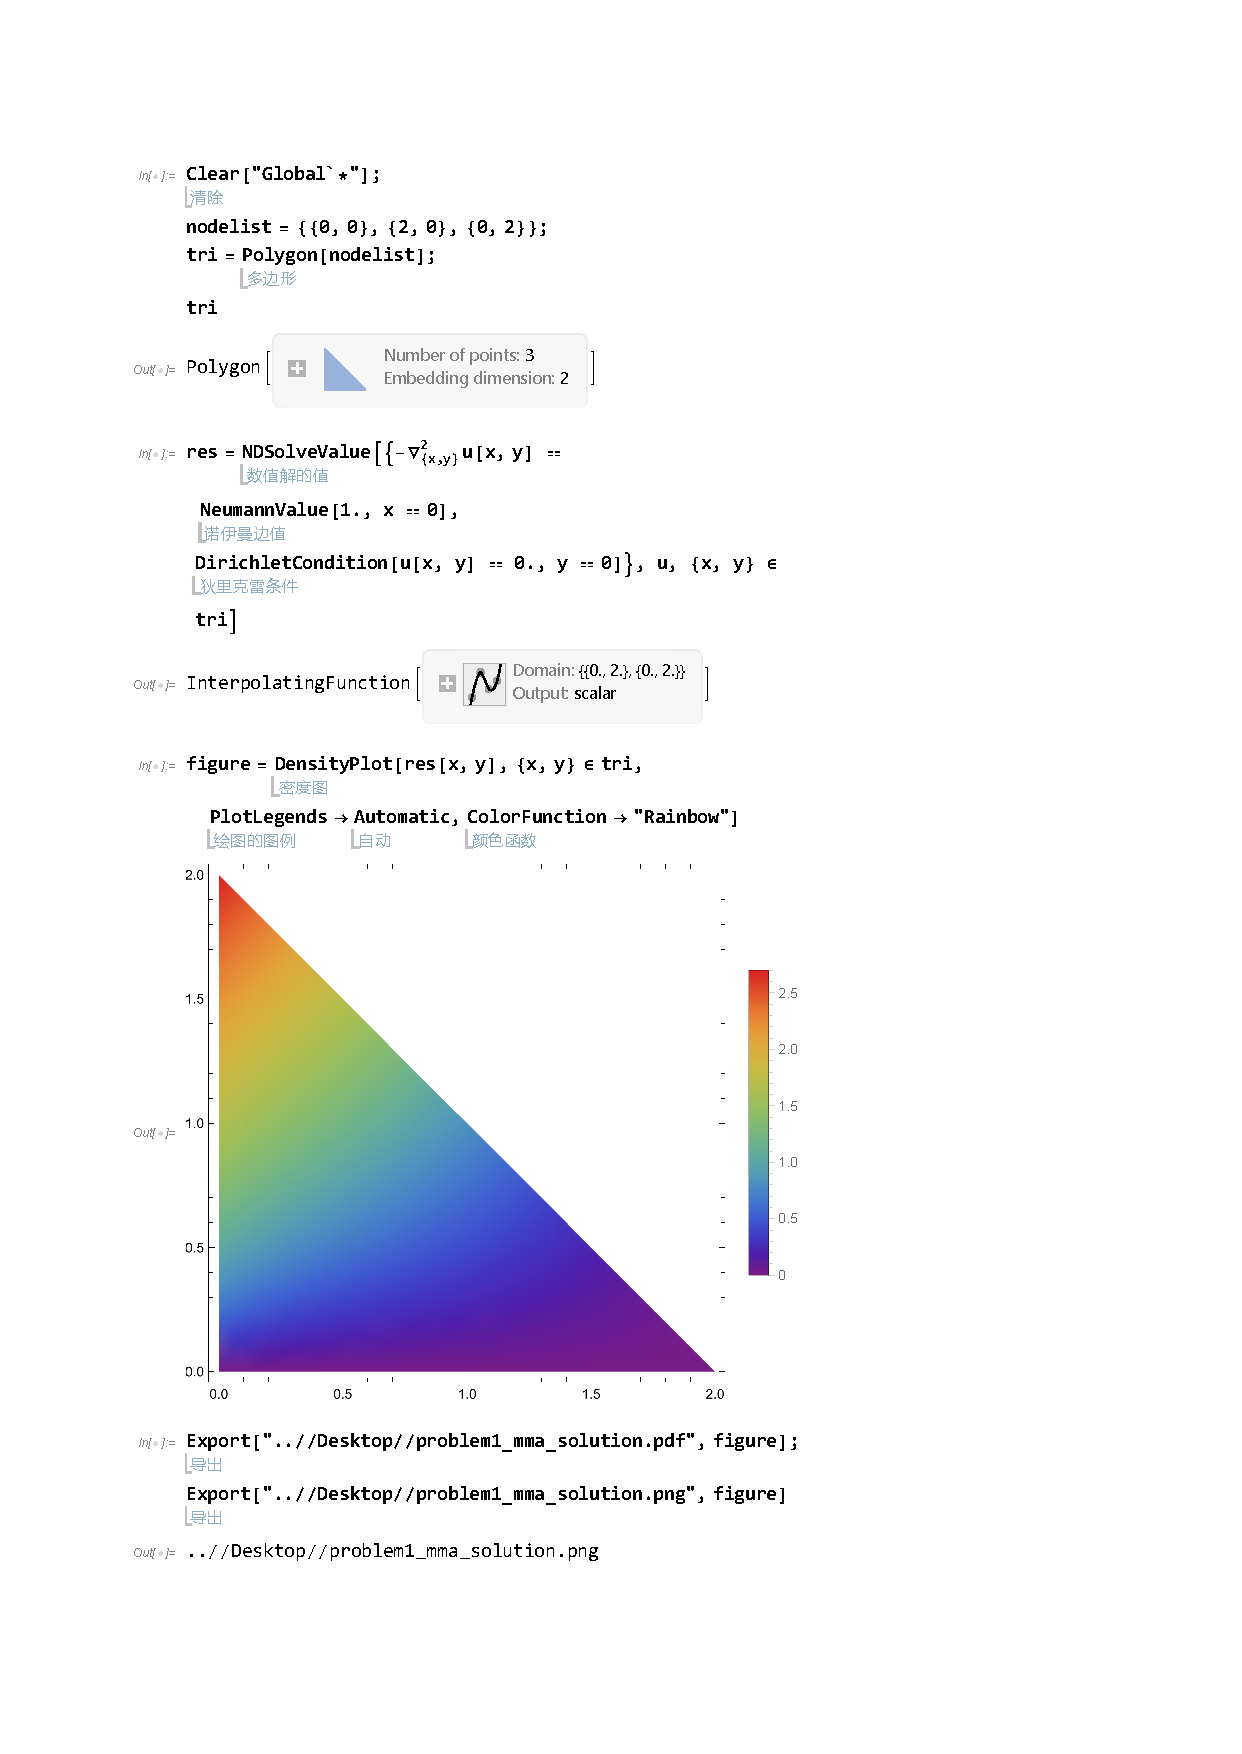
\includepdf[pages=-]{../problem1/mma_solution/problem1.pdf}

\subsubsection{Julia Code Solution}

First we need include the package we use:
\begin{lstlisting}[language=matlab]
using DelaunayTriangulation, CairoMakie;
using SparseArrays, LinearAlgebra;
\end{lstlisting}
here, \verb|DelaunayTriangulation| is used to generate the mesh,
\verb|CairoMakie| is used to plot the mesh and contour.
\verb|SparseArrays| and \verb|LinearAlgebra| are used to solve the linear system.

\begin{figure}[H]
    \centering
    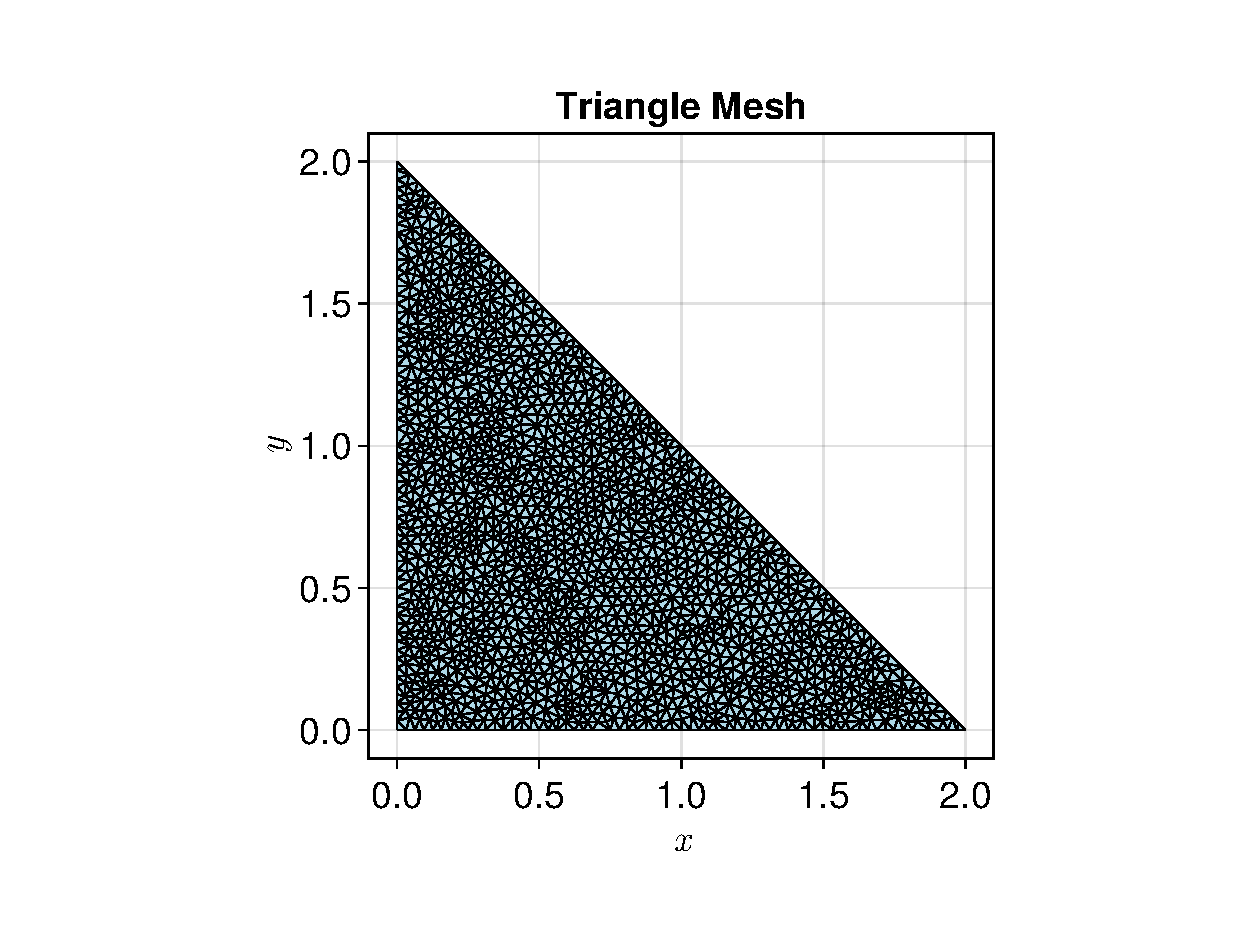
\includegraphics[width=0.6\textwidth]{../problem1/images/triangle_mesh.pdf}
    \caption{Triangle Mesh}
    \label{fig:triangle_mesh}
\end{figure}

Then we define the domain and generate / draw the triangular mesh, 
shown in Fig. \ref{fig:triangle_mesh}.
\begin{lstlisting}[language=matlab]
const triangle_edge_length = 2.;
const max_area = 1e-3;
const min_angle = 31.5;
points = [
    (0., 0.),
    (triangle_edge_length, 0.),
    (0., triangle_edge_length),
    (0., 0.)
];
boundary_nodes, points = convert_boundary_points_to_indices(points);
triangle = triangulate(points; boundary_nodes);
refine!(triangle; max_area=max_area, min_angle=min_angle);

figure = Figure(fontsize=24)
axes = Axis(figure[1, 1], title="Triangle Mesh", titlealign=:center, width=400, height=400, xlabel=L"$x$", ylabel=L"$y$")
triplot!(axes, triangle, triangle_color=:lightblue)
save("triangle_mesh.pdf", figure)
save("triangle_mesh.png", figure)
figure
\end{lstlisting}

In the following code, we generate the stiffness matrix:
\begin{lstlisting}[language=matlab]
function generateStiffnessMatrix(triangle::Triangulation)
    n_nodes = length(triangle.points);
    stiffness_matrix = spzeros(n_nodes, n_nodes);
    for triangle_element in each_triangle(triangle)
        id1, id2, id3 = triangle_element;
        x1, y1 = triangle.points[id1];
        x2, y2 = triangle.points[id2];
        x3, y3 = triangle.points[id3];
        double_area = det(
            [1 x1 y1;
            1 x2 y2;
            1 x3 y3]
        );
        k11 = (x2 - x3)^2 + (y2 - y3)^2;
        k12 = (x1 - x3) * (-x2 + x3) + (y1 - y3) * (-y2 + y3);
        k13 = (x1 - x2) * (x2 - x3) + (y1 - y2) * (y2 - y3);
        k22 = (x1 - x3)^2 + (y1 - y3)^2;
        k23 = (x1 - x2) * (-x1 + x3) + (y1 - y2) * (-y1 + y3);
        k33 = (x1 - x2)^2 + (y1 - y2)^2;
        # first row
        stiffness_matrix[id1, id1] += k11 / double_area / 2;
        stiffness_matrix[id1, id2] += k12 / double_area / 2;
        stiffness_matrix[id1, id3] += k13 / double_area / 2;
        # second row
        stiffness_matrix[id2, id1] += k12 / double_area / 2;
        stiffness_matrix[id2, id2] += k22 / double_area / 2;
        stiffness_matrix[id2, id3] += k23 / double_area / 2;
        # third row
        stiffness_matrix[id3, id1] += k13 / double_area / 2;
        stiffness_matrix[id3, id2] += k23 / double_area / 2;
        stiffness_matrix[id3, id3] += k33 / double_area / 2;
    end
    return stiffness_matrix;
end

stiffness_matrix = generateStiffnessMatrix(triangle);
stiffness_matrix

figure = Figure(fontsize=24)
axes = Axis(figure[1, 1], title="Stiffness Matrix", titlealign=:center, width=400, height=400)
spy!(axes, rotr90(stiffness_matrix), markersize=4, marker=:circle, framecolor=:blue)
hidedecorations!(axes)
save("../images/stiffness_matrix.pdf", figure)
save("../images/stiffness_matrix.png", figure)
figure
\end{lstlisting}

The stiffness matrix is a sparse matrix,
which is shown in Fig. \ref{fig:stiffness_matrix}.
\begin{figure}[H]
    \centering
    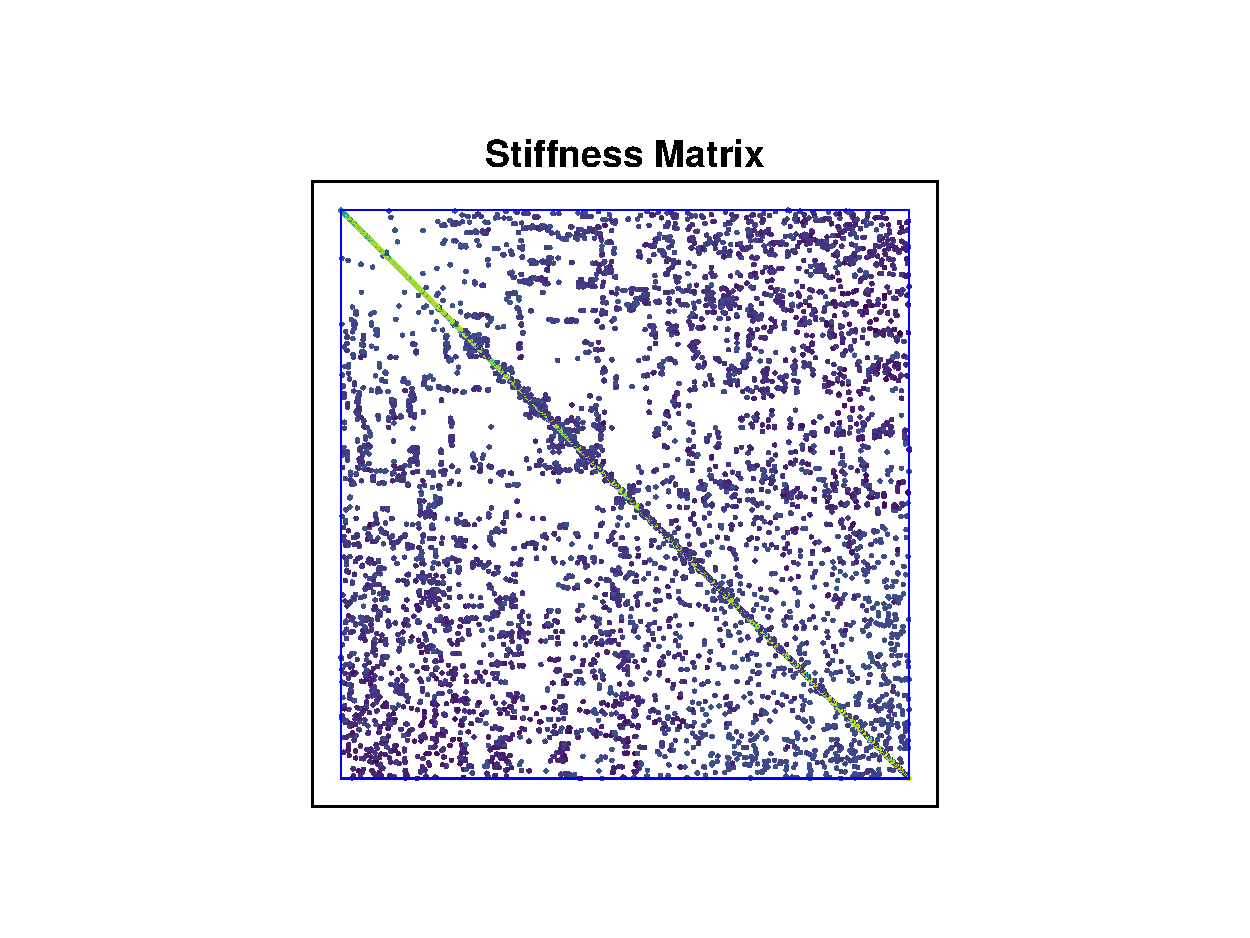
\includegraphics[width=0.6\textwidth]{../problem1/images/stiffness_matrix.pdf}
    \caption{Stiffness Matrix}
    \label{fig:stiffness_matrix}
\end{figure}

For Neumann boundary condition, 
we need to generate the source term vector:
\begin{lstlisting}[language=matlab]
function isLeftBoundaryNode(x, y)
    return x == 0.
end

function generateSourceVector(triangle::Triangulation, neumann_boundary_value::Float64)
    n_nodes = length(triangle.points);
    source_vector = zeros(n_nodes);
    for triangle_element in each_triangle(triangle)
        boundary_nodes = [];
        id1, id2, id3 = triangle_element;
        x1, y1 = triangle.points[id1];
        x2, y2 = triangle.points[id2];
        x3, y3 = triangle.points[id3];
        node_dict = Dict(id1 => (x1, y1), id2 => (x2, y2), id3 => (x3, y3));
        for (id, (x, y)) in node_dict
            if isLeftBoundaryNode(x, y)
                push!(boundary_nodes, id);
            end
        end
        if length(boundary_nodes) == 2
            n1_id, n2_id = boundary_nodes;
            n1_x, n1_y = node_dict[n1_id];
            n2_x, n2_y = node_dict[n2_id];
            edge_length = sqrt((n1_x - n2_x)^2 + (n1_y - n2_y)^2);
            source_vector[n1_id] += neumann_boundary_value * edge_length / 2;
            source_vector[n2_id] += neumann_boundary_value * edge_length / 2;
        else
            continue;
        end
    end
    return source_vector;
end
source_vector = generateSourceVector(triangle, 1.);
\end{lstlisting}

The linear problem has Dirichlet boundary condition,
thus we need to modify the stiffness matrix and source vector.
Below code is fit for the problem with Dirichlet boundary condition:
\begin{lstlisting}[language=matlab]
function solve(
    stiffness_matrix::SparseMatrixCSC, 
    source_vector::Vector, 
    known_nodes_ids::Vector,
    known_nodes_values::Vector
)::Vector
    @assert length(known_nodes_ids) == length(known_nodes_values);
    n_nodes = length(source_vector);
    solution_vector = zeros(n_nodes);
    solution_vector[known_nodes_ids] .= known_nodes_values;
    unknown_nodes_ids = setdiff(1:n_nodes, known_nodes_ids);
    part_stiffness_matrix = stiffness_matrix[unknown_nodes_ids, unknown_nodes_ids];
    part_source_vector = (source_vector .- stiffness_matrix * solution_vector)[unknown_nodes_ids];
    solution_vector[unknown_nodes_ids] .= part_stiffness_matrix \ part_source_vector;
    return solution_vector;
end
\end{lstlisting}

Then we need to get the bottom nodes ID and put them to function above:
\begin{lstlisting}[language=matlab]
function isBottomBoundaryNode(x, y)
    return y == 0.;
end

known_nodes_ids = [];
known_nodes_values = [];
for (id, (x, y)) in enumerate(triangle.points)
    if isBottomBoundaryNode(x, y)
        push!(known_nodes_ids, id);
        push!(known_nodes_values, 0.);
    else
        continue;
    end
end
solution_vector = solve(stiffness_matrix, source_vector, known_nodes_ids, known_nodes_values);
\end{lstlisting}

Finally, we plot the solution:
\begin{lstlisting}[language=matlab]
figure = Figure(fontsize=24)
axes = Axis(figure[1, 1], title="Solution", titlealign=:center, width=400, height=400, xlabel=L"$x$", ylabel=L"$y$")
tr = tricontourf!(axes, triangle, levels=51, solution_vector, colormap=:gist_rainbow)
Colorbar(figure[1, 2], tr, label="Colorbar", labelpadding=10, width=20, height=400)
save("../images/solution.pdf", figure)
save("../images/solution.png", figure)
figure
\end{lstlisting}

The solution is shown in Fig. \ref{fig:solution},
which is consistent with the solution by Mathematica.
What's more, 
the detailed code can be found in folder \verb|problem1/src/solution.jl| or 
\verb|problem1/draft/solution.ipynb|.
To run the code,
you need to install Julia and the packages we use.
And the package \verb|CairoMakie| may take a long time to compile while being imported.
\begin{figure}[H]
    \centering
    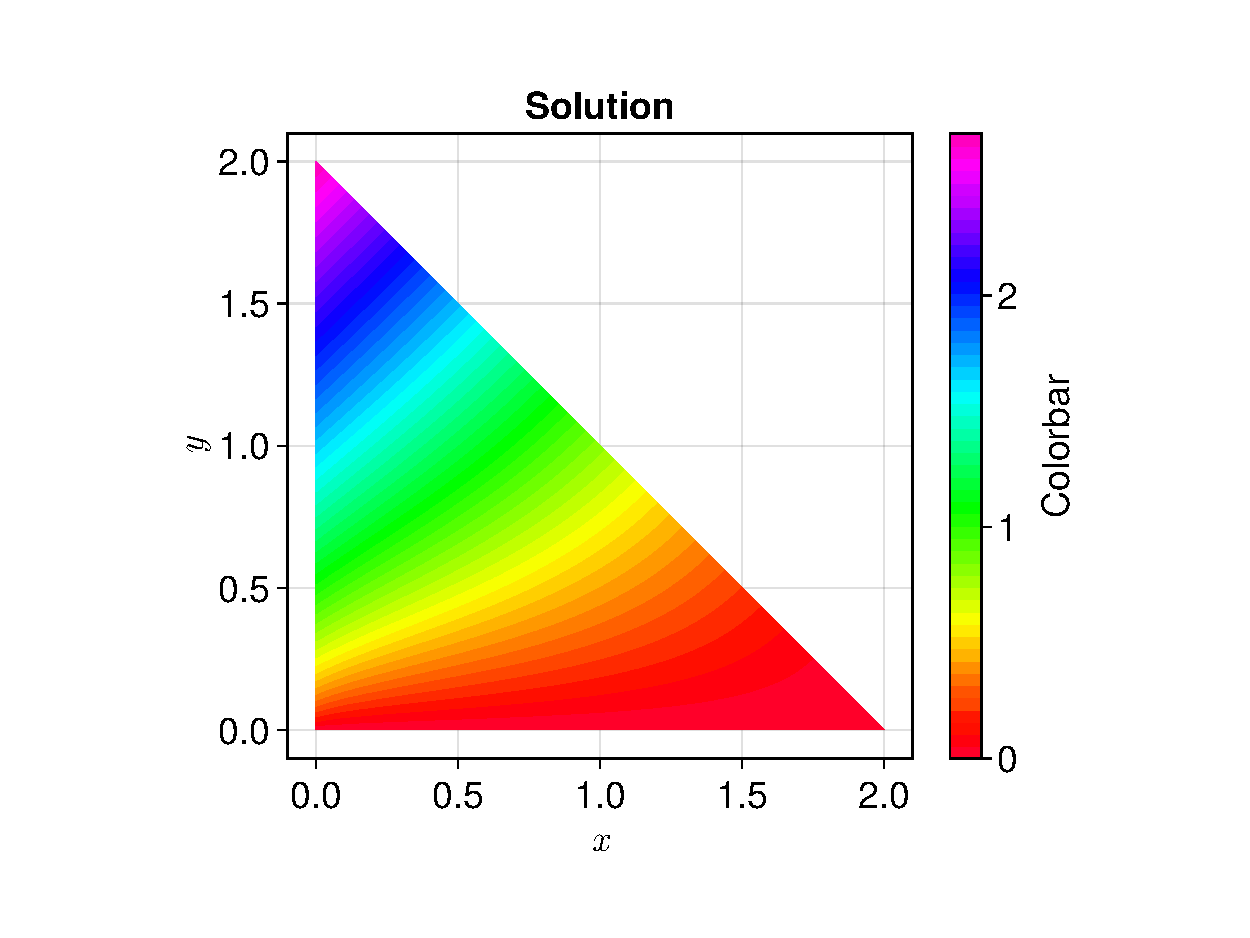
\includegraphics[width=\textwidth]{../problem1/images/solution.pdf}
    \caption{Solution of Problem 1}
    \label{fig:solution}
\end{figure}